\documentclass[tikz, border=2mm]{standalone}
\usetikzlibrary{shapes.misc}

\tikzset{cross/.style={cross out, draw=black, minimum size=2*(#1-\pgflinewidth), inner sep=0pt, outer sep=0pt},
%default radius will be 1pt. 
cross/.default={1pt}}

\begin{document}
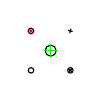
\begin{tikzpicture}[]

\draw (0,0) circle (1pt);

\draw (.5,0) node[cross,rotate=10] {};
\draw (.5,0) circle (1pt);

\draw (0,.5) circle (1pt);
\draw (0,.5) node[cross,red] {};

\draw (.5,.5) node[cross,rotate=30] {};

\draw (0.25,.25) circle (2pt);
\draw (0.25,.25) node[cross=2pt,rotate=45,green]{};
\end{tikzpicture}
\end{document}